% Created by tikzDevice version 0.11 on 2018-04-26 09:26:06
% !TEX encoding = UTF-8 Unicode
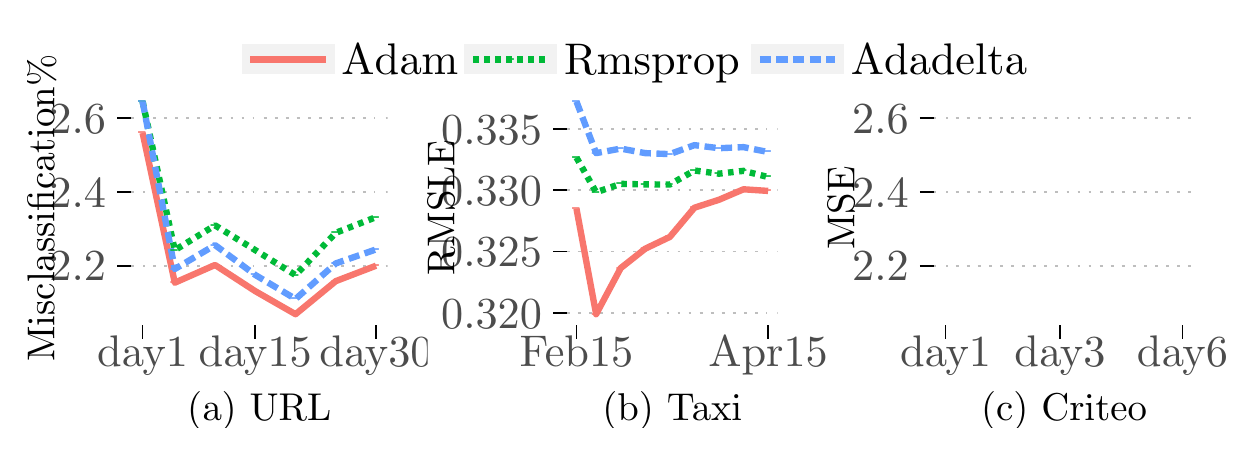
\begin{tikzpicture}[x=1pt,y=1pt]
\definecolor{fillColor}{RGB}{255,255,255}
\path[use as bounding box,fill=fillColor,fill opacity=0.00] (0,0) rectangle (433.62,144.54);
\begin{scope}
\path[clip] (  0.00,  0.00) rectangle (433.62,144.54);
\definecolor{fillColor}{RGB}{255,255,255}

\path[fill=fillColor] ( 67.06,121.66) rectangle (366.56,144.54);
\end{scope}
\begin{scope}
\path[clip] (  0.00,  0.00) rectangle (433.62,144.54);
\definecolor{drawColor}{RGB}{0,0,0}

\node[text=drawColor,anchor=base west,inner sep=0pt, outer sep=0pt, scale=  0.00] at ( 72.75,133.10) {Adaptation};
\end{scope}
\begin{scope}
\path[clip] (  0.00,  0.00) rectangle (433.62,144.54);
\definecolor{drawColor}{RGB}{255,255,255}
\definecolor{fillColor}{gray}{0.95}

\path[draw=drawColor,line width= 0.6pt,line join=round,line cap=round,fill=fillColor] ( 77.09,127.35) rectangle (111.23,138.85);
\end{scope}
\begin{scope}
\path[clip] (  0.00,  0.00) rectangle (433.62,144.54);
\definecolor{drawColor}{RGB}{248,118,109}

\path[draw=drawColor,line width= 2.3pt,line join=round] ( 80.51,133.10) -- (107.82,133.10);
\end{scope}
\begin{scope}
\path[clip] (  0.00,  0.00) rectangle (433.62,144.54);
\definecolor{drawColor}{RGB}{248,118,109}

\node[text=drawColor,anchor=base,inner sep=0pt, outer sep=0pt, scale=  1.00] at ( 94.16,130.94) {-};
\end{scope}
\begin{scope}
\path[clip] (  0.00,  0.00) rectangle (433.62,144.54);
\definecolor{drawColor}{RGB}{255,255,255}
\definecolor{fillColor}{gray}{0.95}

\path[draw=drawColor,line width= 0.6pt,line join=round,line cap=round,fill=fillColor] (157.52,127.35) rectangle (191.67,138.85);
\end{scope}
\begin{scope}
\path[clip] (  0.00,  0.00) rectangle (433.62,144.54);
\definecolor{drawColor}{RGB}{0,186,56}

\path[draw=drawColor,line width= 2.3pt,dash pattern=on 2pt off 2pt ,line join=round] (160.94,133.10) -- (188.25,133.10);
\end{scope}
\begin{scope}
\path[clip] (  0.00,  0.00) rectangle (433.62,144.54);
\definecolor{drawColor}{RGB}{0,186,56}

\node[text=drawColor,anchor=base,inner sep=0pt, outer sep=0pt, scale=  1.00] at (174.60,130.94) {-};
\end{scope}
\begin{scope}
\path[clip] (  0.00,  0.00) rectangle (433.62,144.54);
\definecolor{drawColor}{RGB}{255,255,255}
\definecolor{fillColor}{gray}{0.95}

\path[draw=drawColor,line width= 0.6pt,line join=round,line cap=round,fill=fillColor] (261.15,127.35) rectangle (295.30,138.85);
\end{scope}
\begin{scope}
\path[clip] (  0.00,  0.00) rectangle (433.62,144.54);
\definecolor{drawColor}{RGB}{97,156,255}

\path[draw=drawColor,line width= 2.3pt,dash pattern=on 4pt off 2pt ,line join=round] (264.57,133.10) -- (291.88,133.10);
\end{scope}
\begin{scope}
\path[clip] (  0.00,  0.00) rectangle (433.62,144.54);
\definecolor{drawColor}{RGB}{97,156,255}

\node[text=drawColor,anchor=base,inner sep=0pt, outer sep=0pt, scale=  1.00] at (278.22,130.94) {-};
\end{scope}
\begin{scope}
\path[clip] (  0.00,  0.00) rectangle (433.62,144.54);
\definecolor{drawColor}{RGB}{0,0,0}

\node[text=drawColor,anchor=base west,inner sep=0pt, outer sep=0pt, scale=  1.60] at (113.40,127.59) {Adam};
\end{scope}
\begin{scope}
\path[clip] (  0.00,  0.00) rectangle (433.62,144.54);
\definecolor{drawColor}{RGB}{0,0,0}

\node[text=drawColor,anchor=base west,inner sep=0pt, outer sep=0pt, scale=  1.60] at (193.84,127.59) {Rmsprop};
\end{scope}
\begin{scope}
\path[clip] (  0.00,  0.00) rectangle (433.62,144.54);
\definecolor{drawColor}{RGB}{0,0,0}

\node[text=drawColor,anchor=base west,inner sep=0pt, outer sep=0pt, scale=  1.60] at (297.46,127.59) {Adadelta};
\end{scope}
\begin{scope}
\path[clip] (  0.00,  0.00) rectangle (144.54,121.66);
\definecolor{drawColor}{RGB}{255,255,255}
\definecolor{fillColor}{RGB}{255,255,255}

\path[draw=drawColor,line width= 0.6pt,line join=round,line cap=round,fill=fillColor] (  0.00,  0.00) rectangle (144.54,121.66);
\end{scope}
\begin{scope}
\path[clip] ( 37.31, 37.15) rectangle (130.09,121.66);
\definecolor{fillColor}{RGB}{255,255,255}

\path[fill=fillColor] ( 37.31, 37.15) rectangle (130.09,121.66);
\definecolor{drawColor}{RGB}{255,255,255}

\path[draw=drawColor,line width= 0.3pt,line join=round] ( 37.31, 45.19) --
	(130.09, 45.19);

\path[draw=drawColor,line width= 0.3pt,line join=round] ( 37.31, 71.85) --
	(130.09, 71.85);

\path[draw=drawColor,line width= 0.3pt,line join=round] ( 37.31, 98.50) --
	(130.09, 98.50);

\path[draw=drawColor,line width= 0.3pt,line join=round] ( 61.89, 37.15) --
	( 61.89,121.66);

\path[draw=drawColor,line width= 0.3pt,line join=round] (104.06, 37.15) --
	(104.06,121.66);
\definecolor{drawColor}{RGB}{190,190,190}

\path[draw=drawColor,line width= 0.6pt,dash pattern=on 1pt off 3pt ,line join=round] ( 37.31, 58.52) --
	(130.09, 58.52);

\path[draw=drawColor,line width= 0.6pt,dash pattern=on 1pt off 3pt ,line join=round] ( 37.31, 85.17) --
	(130.09, 85.17);

\path[draw=drawColor,line width= 0.6pt,dash pattern=on 1pt off 3pt ,line join=round] ( 37.31,111.82) --
	(130.09,111.82);
\definecolor{drawColor}{RGB}{255,255,255}

\path[draw=drawColor,line width= 0.6pt,line join=round] ( 41.53, 37.15) --
	( 41.53,121.66);

\path[draw=drawColor,line width= 0.6pt,line join=round] ( 82.24, 37.15) --
	( 82.24,121.66);

\path[draw=drawColor,line width= 0.6pt,line join=round] (125.87, 37.15) --
	(125.87,121.66);
\definecolor{drawColor}{RGB}{248,118,109}

\path[draw=drawColor,line width= 2.3pt,line join=round] ( 41.53,106.49) --
	( 53.16, 52.39) --
	( 67.70, 58.79) --
	( 82.24, 49.33) --
	( 96.79, 41.00) --
	(111.33, 52.95) --
	(125.87, 58.52);
\definecolor{drawColor}{RGB}{0,186,56}

\path[draw=drawColor,line width= 2.3pt,dash pattern=on 2pt off 2pt ,line join=round] ( 41.53,117.82) --
	( 53.16, 64.12) --
	( 67.70, 73.11) --
	( 82.24, 64.16) --
	( 96.79, 55.12) --
	(111.33, 70.41) --
	(125.87, 76.07);
\definecolor{drawColor}{RGB}{97,156,255}

\path[draw=drawColor,line width= 2.3pt,dash pattern=on 4pt off 2pt ,line join=round] ( 41.53,117.82) --
	( 53.16, 57.32) --
	( 67.70, 65.98) --
	( 82.24, 55.19) --
	( 96.79, 46.49) --
	(111.33, 59.35) --
	(125.87, 64.41);
\definecolor{drawColor}{RGB}{248,118,109}

\node[text=drawColor,anchor=base,inner sep=0pt, outer sep=0pt, scale=  1.00] at ( 41.53,104.33) {-};

\node[text=drawColor,anchor=base,inner sep=0pt, outer sep=0pt, scale=  1.00] at ( 53.16, 50.23) {-};

\node[text=drawColor,anchor=base,inner sep=0pt, outer sep=0pt, scale=  1.00] at ( 67.70, 56.62) {-};

\node[text=drawColor,anchor=base,inner sep=0pt, outer sep=0pt, scale=  1.00] at ( 82.24, 47.16) {-};

\node[text=drawColor,anchor=base,inner sep=0pt, outer sep=0pt, scale=  1.00] at ( 96.79, 38.83) {-};

\node[text=drawColor,anchor=base,inner sep=0pt, outer sep=0pt, scale=  1.00] at (111.33, 50.79) {-};

\node[text=drawColor,anchor=base,inner sep=0pt, outer sep=0pt, scale=  1.00] at (125.87, 56.36) {-};
\definecolor{drawColor}{RGB}{0,186,56}

\node[text=drawColor,anchor=base,inner sep=0pt, outer sep=0pt, scale=  1.00] at ( 41.53,115.66) {-};

\node[text=drawColor,anchor=base,inner sep=0pt, outer sep=0pt, scale=  1.00] at ( 53.16, 61.95) {-};

\node[text=drawColor,anchor=base,inner sep=0pt, outer sep=0pt, scale=  1.00] at ( 67.70, 70.95) {-};

\node[text=drawColor,anchor=base,inner sep=0pt, outer sep=0pt, scale=  1.00] at ( 82.24, 62.00) {-};

\node[text=drawColor,anchor=base,inner sep=0pt, outer sep=0pt, scale=  1.00] at ( 96.79, 52.96) {-};

\node[text=drawColor,anchor=base,inner sep=0pt, outer sep=0pt, scale=  1.00] at (111.33, 68.24) {-};

\node[text=drawColor,anchor=base,inner sep=0pt, outer sep=0pt, scale=  1.00] at (125.87, 73.90) {-};
\definecolor{drawColor}{RGB}{97,156,255}

\node[text=drawColor,anchor=base,inner sep=0pt, outer sep=0pt, scale=  1.00] at ( 41.53,115.66) {-};

\node[text=drawColor,anchor=base,inner sep=0pt, outer sep=0pt, scale=  1.00] at ( 53.16, 55.16) {-};

\node[text=drawColor,anchor=base,inner sep=0pt, outer sep=0pt, scale=  1.00] at ( 67.70, 63.82) {-};

\node[text=drawColor,anchor=base,inner sep=0pt, outer sep=0pt, scale=  1.00] at ( 82.24, 53.03) {-};

\node[text=drawColor,anchor=base,inner sep=0pt, outer sep=0pt, scale=  1.00] at ( 96.79, 44.33) {-};

\node[text=drawColor,anchor=base,inner sep=0pt, outer sep=0pt, scale=  1.00] at (111.33, 57.18) {-};

\node[text=drawColor,anchor=base,inner sep=0pt, outer sep=0pt, scale=  1.00] at (125.87, 62.24) {-};
\end{scope}
\begin{scope}
\path[clip] (  0.00,  0.00) rectangle (433.62,144.54);
\definecolor{drawColor}{gray}{0.30}

\node[text=drawColor,anchor=base east,inner sep=0pt, outer sep=0pt, scale=  1.60] at ( 28.31, 53.01) {2.2};

\node[text=drawColor,anchor=base east,inner sep=0pt, outer sep=0pt, scale=  1.60] at ( 28.31, 79.66) {2.4};

\node[text=drawColor,anchor=base east,inner sep=0pt, outer sep=0pt, scale=  1.60] at ( 28.31,106.31) {2.6};
\end{scope}
\begin{scope}
\path[clip] (  0.00,  0.00) rectangle (433.62,144.54);
\definecolor{drawColor}{RGB}{0,0,0}

\path[draw=drawColor,line width= 0.6pt,line join=round] ( 32.31, 58.52) --
	( 37.31, 58.52);

\path[draw=drawColor,line width= 0.6pt,line join=round] ( 32.31, 85.17) --
	( 37.31, 85.17);

\path[draw=drawColor,line width= 0.6pt,line join=round] ( 32.31,111.82) --
	( 37.31,111.82);
\end{scope}
\begin{scope}
\path[clip] (  0.00,  0.00) rectangle (433.62,144.54);
\definecolor{drawColor}{RGB}{0,0,0}

\path[draw=drawColor,line width= 0.6pt,line join=round] ( 41.53, 32.15) --
	( 41.53, 37.15);

\path[draw=drawColor,line width= 0.6pt,line join=round] ( 82.24, 32.15) --
	( 82.24, 37.15);

\path[draw=drawColor,line width= 0.6pt,line join=round] (125.87, 32.15) --
	(125.87, 37.15);
\end{scope}
\begin{scope}
\path[clip] (  0.00,  0.00) rectangle (433.62,144.54);
\definecolor{drawColor}{gray}{0.30}

\node[text=drawColor,anchor=base,inner sep=0pt, outer sep=0pt, scale=  1.60] at ( 41.53, 22.14) {day1};

\node[text=drawColor,anchor=base,inner sep=0pt, outer sep=0pt, scale=  1.60] at ( 82.24, 22.14) {day15};

\node[text=drawColor,anchor=base,inner sep=0pt, outer sep=0pt, scale=  1.60] at (125.87, 22.14) {day30};
\end{scope}
\begin{scope}
\path[clip] (  0.00,  0.00) rectangle (433.62,144.54);
\definecolor{drawColor}{RGB}{0,0,0}

\node[text=drawColor,anchor=base,inner sep=0pt, outer sep=0pt, scale=  1.40] at ( 83.70,  2.49) {(a) URL};
\end{scope}
\begin{scope}
\path[clip] (  0.00,  0.00) rectangle (433.62,144.54);
\definecolor{drawColor}{RGB}{0,0,0}

\node[text=drawColor,rotate= 90.00,anchor=base,inner sep=0pt, outer sep=0pt, scale=  1.40] at (  9.64, 79.41) {Misclassification\%};
\end{scope}
\begin{scope}
\path[clip] (144.54,  0.00) rectangle (289.08,121.66);
\definecolor{drawColor}{RGB}{255,255,255}
\definecolor{fillColor}{RGB}{255,255,255}

\path[draw=drawColor,line width= 0.6pt,line join=round,line cap=round,fill=fillColor] (144.54,  0.00) rectangle (289.08,121.66);
\end{scope}
\begin{scope}
\path[clip] (194.85, 37.15) rectangle (271.01,121.66);
\definecolor{fillColor}{RGB}{255,255,255}

\path[fill=fillColor] (194.85, 37.15) rectangle (271.01,121.66);
\definecolor{drawColor}{RGB}{255,255,255}

\path[draw=drawColor,line width= 0.3pt,line join=round] (194.85, 52.50) --
	(271.01, 52.50);

\path[draw=drawColor,line width= 0.3pt,line join=round] (194.85, 74.70) --
	(271.01, 74.70);

\path[draw=drawColor,line width= 0.3pt,line join=round] (194.85, 96.90) --
	(271.01, 96.90);

\path[draw=drawColor,line width= 0.3pt,line join=round] (194.85,119.10) --
	(271.01,119.10);

\path[draw=drawColor,line width= 0.3pt,line join=round] (232.93, 37.15) --
	(232.93,121.66);
\definecolor{drawColor}{RGB}{190,190,190}

\path[draw=drawColor,line width= 0.6pt,dash pattern=on 1pt off 3pt ,line join=round] (194.85, 41.40) --
	(271.01, 41.40);

\path[draw=drawColor,line width= 0.6pt,dash pattern=on 1pt off 3pt ,line join=round] (194.85, 63.60) --
	(271.01, 63.60);

\path[draw=drawColor,line width= 0.6pt,dash pattern=on 1pt off 3pt ,line join=round] (194.85, 85.80) --
	(271.01, 85.80);

\path[draw=drawColor,line width= 0.6pt,dash pattern=on 1pt off 3pt ,line join=round] (194.85,108.00) --
	(271.01,108.00);
\definecolor{drawColor}{RGB}{255,255,255}

\path[draw=drawColor,line width= 0.6pt,line join=round] (198.31, 37.15) --
	(198.31,121.66);

\path[draw=drawColor,line width= 0.6pt,line join=round] (267.55, 37.15) --
	(267.55,121.66);
\definecolor{drawColor}{RGB}{248,118,109}

\path[draw=drawColor,line width= 2.3pt,line join=round] (198.31, 79.10) --
	(205.41, 41.00) --
	(214.29, 57.66) --
	(223.16, 64.68) --
	(232.04, 68.92) --
	(240.92, 79.48) --
	(249.80, 82.35) --
	(258.67, 86.14) --
	(267.55, 85.55);
\definecolor{drawColor}{RGB}{0,186,56}

\path[draw=drawColor,line width= 2.3pt,dash pattern=on 2pt off 2pt ,line join=round] (198.31, 97.60) --
	(205.41, 85.07) --
	(214.29, 88.10) --
	(223.16, 87.91) --
	(232.04, 87.87) --
	(240.92, 92.92) --
	(249.80, 91.78) --
	(258.67, 92.80) --
	(267.55, 90.58);
\definecolor{drawColor}{RGB}{97,156,255}

\path[draw=drawColor,line width= 2.3pt,dash pattern=on 4pt off 2pt ,line join=round] (198.31,117.82) --
	(205.41, 99.21) --
	(214.29,100.84) --
	(223.16, 99.21) --
	(232.04, 98.85) --
	(240.92,102.09) --
	(249.80,100.98) --
	(258.67,101.37) --
	(267.55, 99.61);
\definecolor{drawColor}{RGB}{248,118,109}

\node[text=drawColor,anchor=base,inner sep=0pt, outer sep=0pt, scale=  1.00] at (198.31, 76.93) {-};

\node[text=drawColor,anchor=base,inner sep=0pt, outer sep=0pt, scale=  1.00] at (205.41, 38.83) {-};

\node[text=drawColor,anchor=base,inner sep=0pt, outer sep=0pt, scale=  1.00] at (214.29, 55.49) {-};

\node[text=drawColor,anchor=base,inner sep=0pt, outer sep=0pt, scale=  1.00] at (223.16, 62.52) {-};

\node[text=drawColor,anchor=base,inner sep=0pt, outer sep=0pt, scale=  1.00] at (232.04, 66.76) {-};

\node[text=drawColor,anchor=base,inner sep=0pt, outer sep=0pt, scale=  1.00] at (240.92, 77.32) {-};

\node[text=drawColor,anchor=base,inner sep=0pt, outer sep=0pt, scale=  1.00] at (249.80, 80.19) {-};

\node[text=drawColor,anchor=base,inner sep=0pt, outer sep=0pt, scale=  1.00] at (258.67, 83.98) {-};

\node[text=drawColor,anchor=base,inner sep=0pt, outer sep=0pt, scale=  1.00] at (267.55, 83.38) {-};
\definecolor{drawColor}{RGB}{0,186,56}

\node[text=drawColor,anchor=base,inner sep=0pt, outer sep=0pt, scale=  1.00] at (198.31, 95.43) {-};

\node[text=drawColor,anchor=base,inner sep=0pt, outer sep=0pt, scale=  1.00] at (205.41, 82.91) {-};

\node[text=drawColor,anchor=base,inner sep=0pt, outer sep=0pt, scale=  1.00] at (214.29, 85.94) {-};

\node[text=drawColor,anchor=base,inner sep=0pt, outer sep=0pt, scale=  1.00] at (223.16, 85.75) {-};

\node[text=drawColor,anchor=base,inner sep=0pt, outer sep=0pt, scale=  1.00] at (232.04, 85.70) {-};

\node[text=drawColor,anchor=base,inner sep=0pt, outer sep=0pt, scale=  1.00] at (240.92, 90.76) {-};

\node[text=drawColor,anchor=base,inner sep=0pt, outer sep=0pt, scale=  1.00] at (249.80, 89.62) {-};

\node[text=drawColor,anchor=base,inner sep=0pt, outer sep=0pt, scale=  1.00] at (258.67, 90.63) {-};

\node[text=drawColor,anchor=base,inner sep=0pt, outer sep=0pt, scale=  1.00] at (267.55, 88.42) {-};
\definecolor{drawColor}{RGB}{97,156,255}

\node[text=drawColor,anchor=base,inner sep=0pt, outer sep=0pt, scale=  1.00] at (198.31,115.66) {-};

\node[text=drawColor,anchor=base,inner sep=0pt, outer sep=0pt, scale=  1.00] at (205.41, 97.04) {-};

\node[text=drawColor,anchor=base,inner sep=0pt, outer sep=0pt, scale=  1.00] at (214.29, 98.68) {-};

\node[text=drawColor,anchor=base,inner sep=0pt, outer sep=0pt, scale=  1.00] at (223.16, 97.05) {-};

\node[text=drawColor,anchor=base,inner sep=0pt, outer sep=0pt, scale=  1.00] at (232.04, 96.69) {-};

\node[text=drawColor,anchor=base,inner sep=0pt, outer sep=0pt, scale=  1.00] at (240.92, 99.93) {-};

\node[text=drawColor,anchor=base,inner sep=0pt, outer sep=0pt, scale=  1.00] at (249.80, 98.82) {-};

\node[text=drawColor,anchor=base,inner sep=0pt, outer sep=0pt, scale=  1.00] at (258.67, 99.21) {-};

\node[text=drawColor,anchor=base,inner sep=0pt, outer sep=0pt, scale=  1.00] at (267.55, 97.45) {-};
\end{scope}
\begin{scope}
\path[clip] (  0.00,  0.00) rectangle (433.62,144.54);
\definecolor{drawColor}{gray}{0.30}

\node[text=drawColor,anchor=base east,inner sep=0pt, outer sep=0pt, scale=  1.60] at (185.85, 35.89) {0.320};

\node[text=drawColor,anchor=base east,inner sep=0pt, outer sep=0pt, scale=  1.60] at (185.85, 58.09) {0.325};

\node[text=drawColor,anchor=base east,inner sep=0pt, outer sep=0pt, scale=  1.60] at (185.85, 80.29) {0.330};

\node[text=drawColor,anchor=base east,inner sep=0pt, outer sep=0pt, scale=  1.60] at (185.85,102.49) {0.335};
\end{scope}
\begin{scope}
\path[clip] (  0.00,  0.00) rectangle (433.62,144.54);
\definecolor{drawColor}{RGB}{0,0,0}

\path[draw=drawColor,line width= 0.6pt,line join=round] (189.85, 41.40) --
	(194.85, 41.40);

\path[draw=drawColor,line width= 0.6pt,line join=round] (189.85, 63.60) --
	(194.85, 63.60);

\path[draw=drawColor,line width= 0.6pt,line join=round] (189.85, 85.80) --
	(194.85, 85.80);

\path[draw=drawColor,line width= 0.6pt,line join=round] (189.85,108.00) --
	(194.85,108.00);
\end{scope}
\begin{scope}
\path[clip] (  0.00,  0.00) rectangle (433.62,144.54);
\definecolor{drawColor}{RGB}{0,0,0}

\path[draw=drawColor,line width= 0.6pt,line join=round] (198.31, 32.15) --
	(198.31, 37.15);

\path[draw=drawColor,line width= 0.6pt,line join=round] (267.55, 32.15) --
	(267.55, 37.15);
\end{scope}
\begin{scope}
\path[clip] (  0.00,  0.00) rectangle (433.62,144.54);
\definecolor{drawColor}{gray}{0.30}

\node[text=drawColor,anchor=base,inner sep=0pt, outer sep=0pt, scale=  1.60] at (198.31, 22.14) {Feb15};

\node[text=drawColor,anchor=base,inner sep=0pt, outer sep=0pt, scale=  1.60] at (267.55, 22.14) {Apr15};
\end{scope}
\begin{scope}
\path[clip] (  0.00,  0.00) rectangle (433.62,144.54);
\definecolor{drawColor}{RGB}{0,0,0}

\node[text=drawColor,anchor=base,inner sep=0pt, outer sep=0pt, scale=  1.40] at (232.93,  2.49) {(b) Taxi};
\end{scope}
\begin{scope}
\path[clip] (  0.00,  0.00) rectangle (433.62,144.54);
\definecolor{drawColor}{RGB}{0,0,0}

\node[text=drawColor,rotate= 90.00,anchor=base,inner sep=0pt, outer sep=0pt, scale=  1.40] at (154.18, 79.41) {RMSLE};
\end{scope}
\begin{scope}
\path[clip] (289.08,  0.00) rectangle (433.62,121.66);
\definecolor{drawColor}{RGB}{255,255,255}
\definecolor{fillColor}{RGB}{255,255,255}

\path[draw=drawColor,line width= 0.6pt,line join=round,line cap=round,fill=fillColor] (289.08,  0.00) rectangle (433.62,121.66);
\end{scope}
\begin{scope}
\path[clip] (327.39, 37.15) rectangle (421.57,121.66);
\definecolor{fillColor}{RGB}{255,255,255}

\path[fill=fillColor] (327.39, 37.15) rectangle (421.57,121.66);
\definecolor{drawColor}{RGB}{255,255,255}

\path[draw=drawColor,line width= 0.3pt,line join=round] (327.39, 45.19) --
	(421.57, 45.19);

\path[draw=drawColor,line width= 0.3pt,line join=round] (327.39, 71.85) --
	(421.57, 71.85);

\path[draw=drawColor,line width= 0.3pt,line join=round] (327.39, 98.50) --
	(421.57, 98.50);

\path[draw=drawColor,line width= 0.3pt,line join=round] (352.34, 37.15) --
	(352.34,121.66);

\path[draw=drawColor,line width= 0.3pt,line join=round] (395.15, 37.15) --
	(395.15,121.66);
\definecolor{drawColor}{RGB}{190,190,190}

\path[draw=drawColor,line width= 0.6pt,dash pattern=on 1pt off 3pt ,line join=round] (327.39, 58.52) --
	(421.57, 58.52);

\path[draw=drawColor,line width= 0.6pt,dash pattern=on 1pt off 3pt ,line join=round] (327.39, 85.17) --
	(421.57, 85.17);

\path[draw=drawColor,line width= 0.6pt,dash pattern=on 1pt off 3pt ,line join=round] (327.39,111.82) --
	(421.57,111.82);
\definecolor{drawColor}{RGB}{255,255,255}

\path[draw=drawColor,line width= 0.6pt,line join=round] (331.67, 37.15) --
	(331.67,121.66);

\path[draw=drawColor,line width= 0.6pt,line join=round] (373.01, 37.15) --
	(373.01,121.66);

\path[draw=drawColor,line width= 0.6pt,line join=round] (417.29, 37.15) --
	(417.29,121.66);
\end{scope}
\begin{scope}
\path[clip] (  0.00,  0.00) rectangle (433.62,144.54);
\definecolor{drawColor}{gray}{0.30}

\node[text=drawColor,anchor=base east,inner sep=0pt, outer sep=0pt, scale=  1.60] at (318.39, 53.01) {2.2};

\node[text=drawColor,anchor=base east,inner sep=0pt, outer sep=0pt, scale=  1.60] at (318.39, 79.66) {2.4};

\node[text=drawColor,anchor=base east,inner sep=0pt, outer sep=0pt, scale=  1.60] at (318.39,106.31) {2.6};
\end{scope}
\begin{scope}
\path[clip] (  0.00,  0.00) rectangle (433.62,144.54);
\definecolor{drawColor}{RGB}{0,0,0}

\path[draw=drawColor,line width= 0.6pt,line join=round] (322.39, 58.52) --
	(327.39, 58.52);

\path[draw=drawColor,line width= 0.6pt,line join=round] (322.39, 85.17) --
	(327.39, 85.17);

\path[draw=drawColor,line width= 0.6pt,line join=round] (322.39,111.82) --
	(327.39,111.82);
\end{scope}
\begin{scope}
\path[clip] (  0.00,  0.00) rectangle (433.62,144.54);
\definecolor{drawColor}{RGB}{0,0,0}

\path[draw=drawColor,line width= 0.6pt,line join=round] (331.67, 32.15) --
	(331.67, 37.15);

\path[draw=drawColor,line width= 0.6pt,line join=round] (373.01, 32.15) --
	(373.01, 37.15);

\path[draw=drawColor,line width= 0.6pt,line join=round] (417.29, 32.15) --
	(417.29, 37.15);
\end{scope}
\begin{scope}
\path[clip] (  0.00,  0.00) rectangle (433.62,144.54);
\definecolor{drawColor}{gray}{0.30}

\node[text=drawColor,anchor=base,inner sep=0pt, outer sep=0pt, scale=  1.60] at (331.67, 22.14) {day1};

\node[text=drawColor,anchor=base,inner sep=0pt, outer sep=0pt, scale=  1.60] at (373.01, 22.14) {day3};

\node[text=drawColor,anchor=base,inner sep=0pt, outer sep=0pt, scale=  1.60] at (417.29, 22.14) {day6};
\end{scope}
\begin{scope}
\path[clip] (  0.00,  0.00) rectangle (433.62,144.54);
\definecolor{drawColor}{RGB}{0,0,0}

\node[text=drawColor,anchor=base,inner sep=0pt, outer sep=0pt, scale=  1.40] at (374.48,  2.49) {(c) Criteo};
\end{scope}
\begin{scope}
\path[clip] (  0.00,  0.00) rectangle (433.62,144.54);
\definecolor{drawColor}{RGB}{0,0,0}

\node[text=drawColor,rotate= 90.00,anchor=base,inner sep=0pt, outer sep=0pt, scale=  1.40] at (298.72, 79.41) {MSE};
\end{scope}
\end{tikzpicture}
